%%%%%%%%%%%%%%%%%%%%%%%%%%%%%%%%%%%%%%%%%%%%%%%%%%%%%%%%%%%%%%%
%2345678901234567890123456789012345678901234567890123456789012345678901234567890
%        1         2         3         4         5         6         7         8

\documentclass[letterpaper, 10 pt, conference]{ieeeconf}  % Comment this line out if you need a4paper

%\documentclass[a4paper, 10pt, conference]{ieeeconf}      % Use this line for a4 paper

\IEEEoverridecommandlockouts                              % This command is only needed if 
                                                          % you want to use the \thanks command

\overrideIEEEmargins                                      % Needed to meet printer requirements.

% See the \addtolength command later in the file to balance the column lengths
% on the last page of the document

% The following packages can be found on http:\\www.ctan.org
\usepackage{graphicx} % for pdf, bitmapped graphics files
%\usepackage{epsfig} % for postscript graphics files
%\usepackage{mathptmx} % assumes new font selection scheme installed
%\usepackage{times} % assumes new font selection scheme installed
\usepackage{amsmath} % assumes amsmath package installed
\usepackage{amsfonts} % assumes amsfonts package installed
%\usepackage{amssymb}  % assumes amsmath package installed

\title{\LARGE \bf {Wavelet Based ROI Lossless Medical Image Watermarking Scheme}}


\author{\it Rui Shen, Pouria Tohidi, Shuwen Wei  \\ % <-this % stops a space
\normalsize {Department of Electrical and Computer Engineering, Johns Hopkins University}
\thanks{520.646 WAVELETS AND FILTER BANKS}}

\begin{document}



\maketitle
\thispagestyle{empty}
\pagestyle{empty}


%%%%%%%%%%%%%%%%%%%%%%%%%%%%%%%%%%%%%%%%%%%%%%%%%%%%%%%%%%%%%%%%%%%%%%%%%%%%%%%%
\begin{abstract}


\end{abstract}


%%%%%%%%%%%%%%%%%%%%%%%%%%%%%%%%%%%%%%%%%%%%%%%%%%%%%%%%%%%%%%%%%%%%%%%%%%%%%%%%
\section{INTRODUCTION}


\section{DATA}


\section{METHODOLOGY}
\subsection{Watermark embedding}
The EPR data was split into several blocks for embedding into different sub-bands of wavelet decomposition levels  (Fig. \ref{WMPos}). The energy of the image is mainly concentrated in the high decomposition level while the low frequency. Among sub-bands in the same level, the diagonal ones contain the least energy which means they are more vulnerable to attack. Embedding the watermark in the diagonal detail in the first level can be used in tamper assessing detection of the image. Compared with the diagonal sub-bands, the horizontal and the vertical ones include higher energy, which can guarantee increased robustness when storing EPR data. However, the coarse approximation contains the most crucial information of the original image and would significantly affect the image quality, this sub-bands should avoid any changing in wavelet coefficients.
\begin{figure}[htbp]
	\centering
	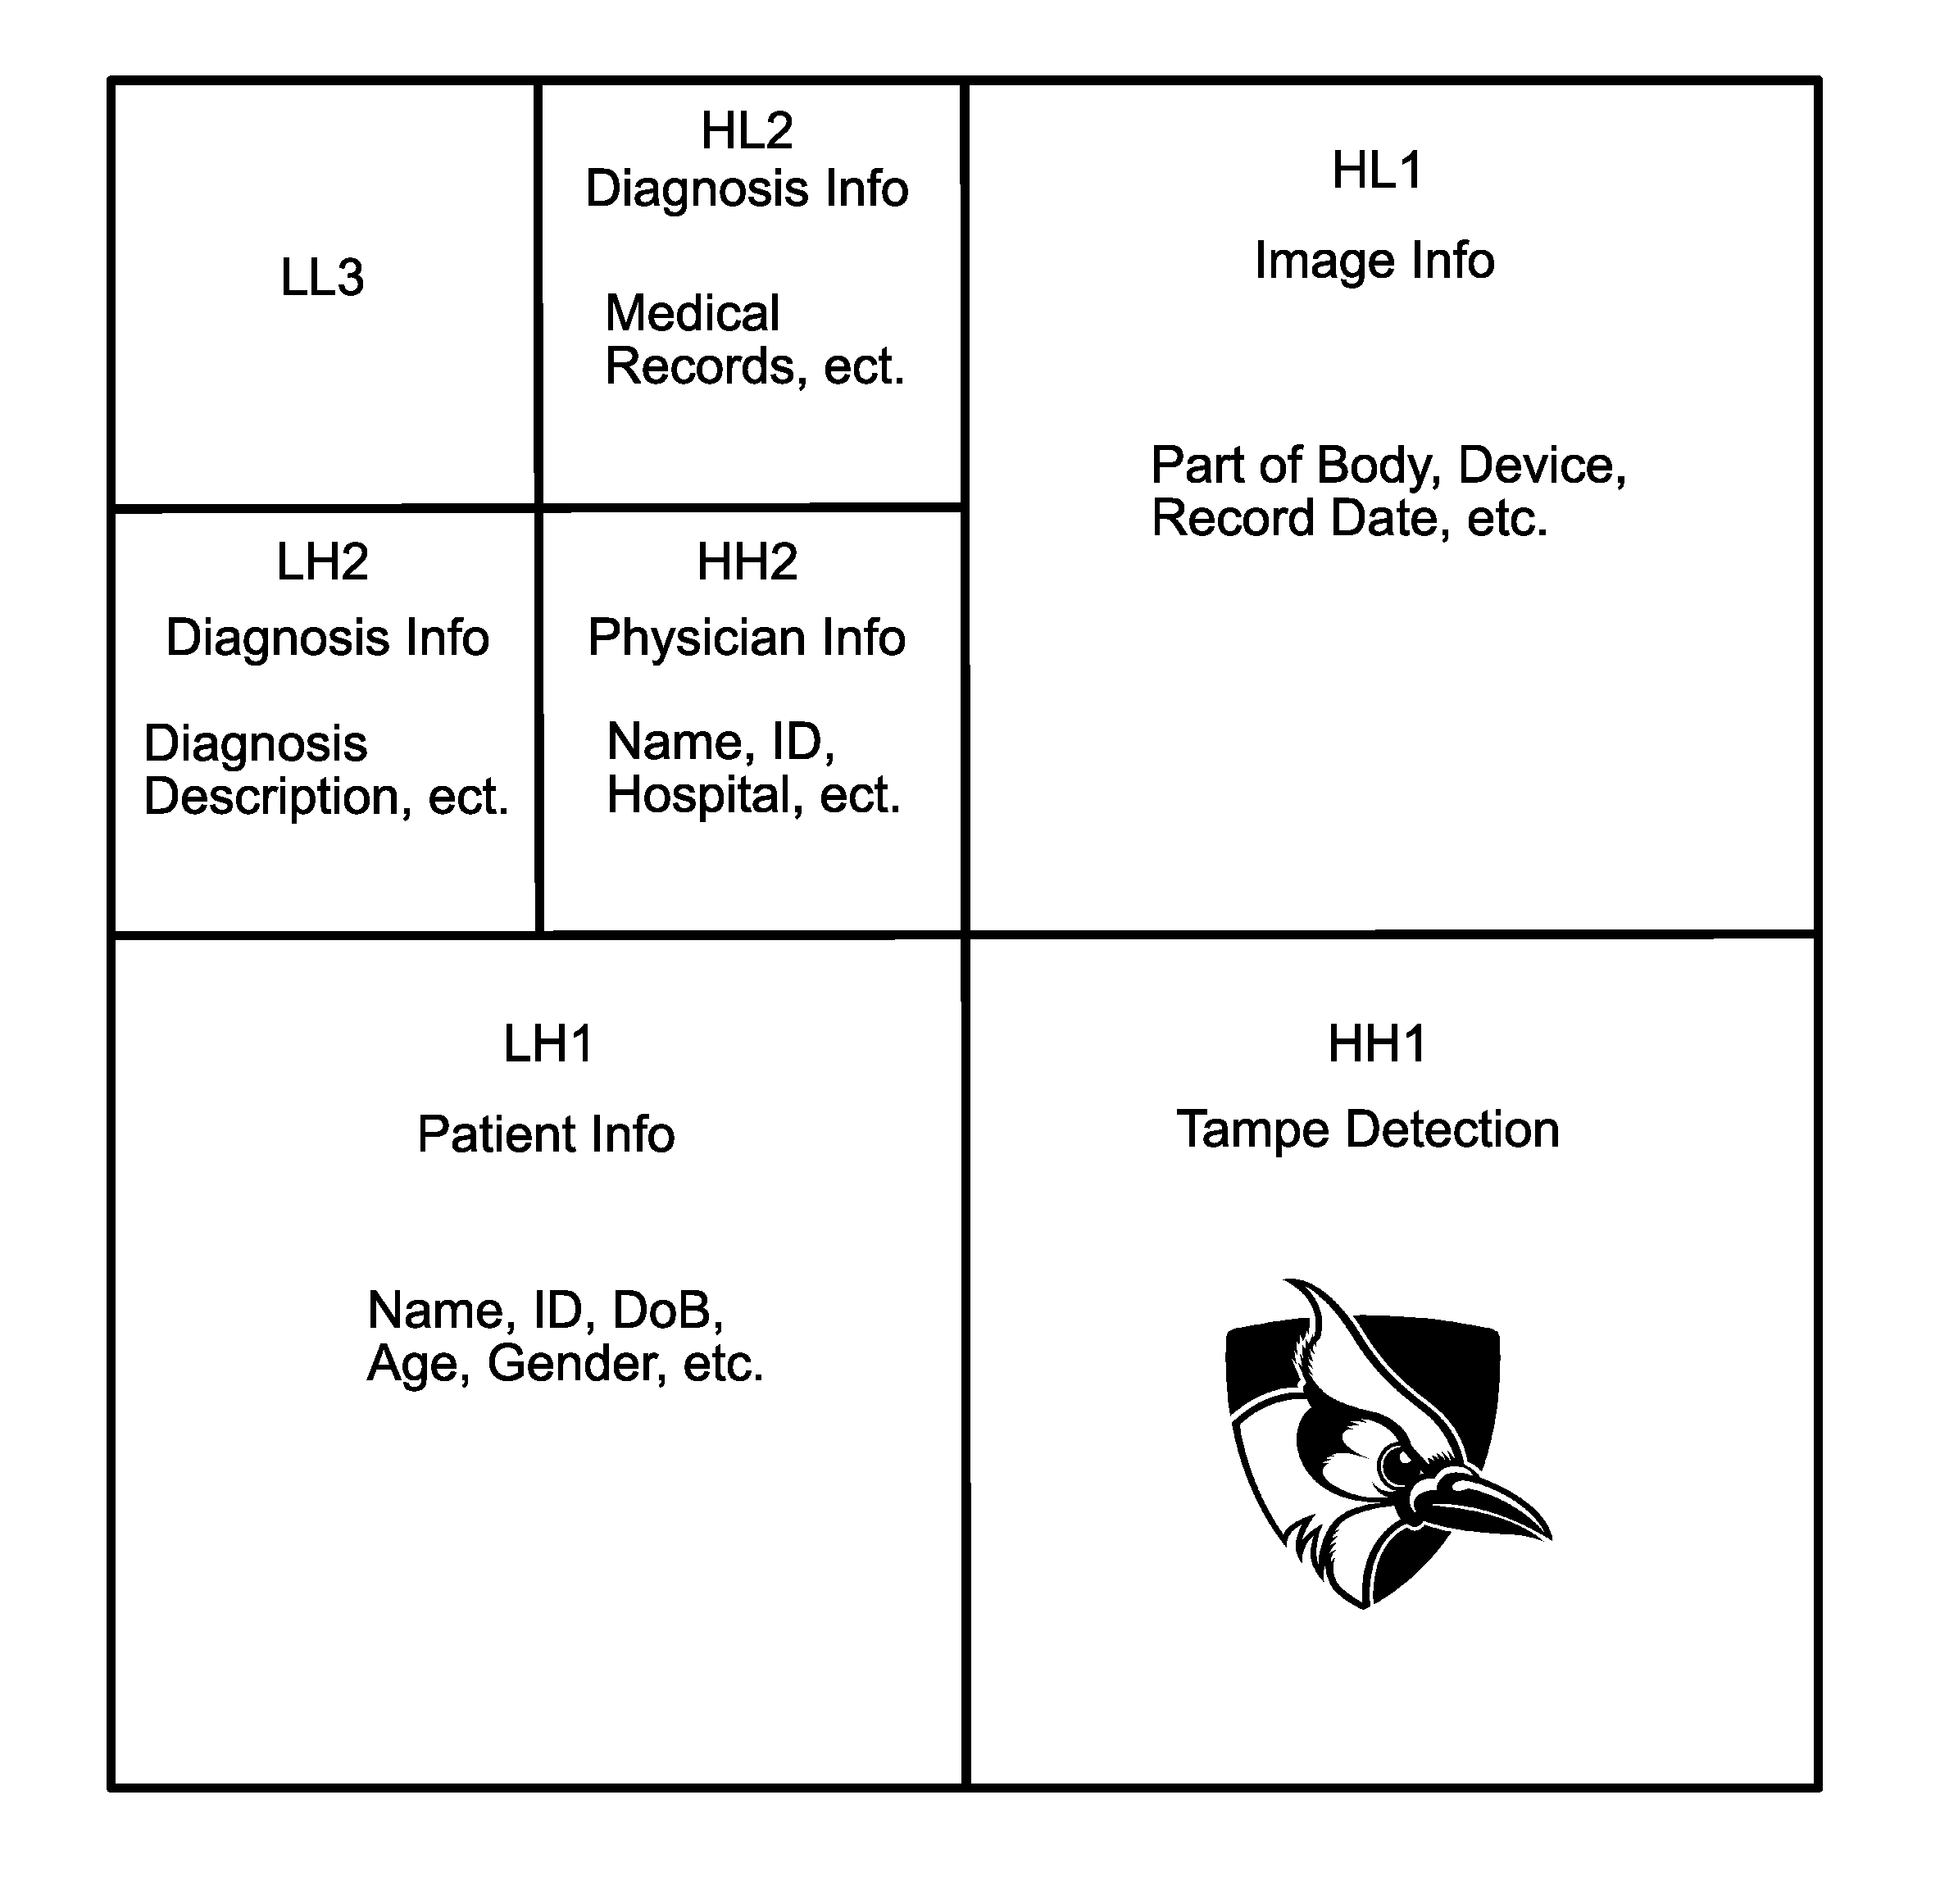
\includegraphics[width=1\linewidth]{WMPos}
	\caption{Structure of 2-level DWT and illustration of watermarking position}
	\label{WMPos}
\end{figure}
\\

\subsection{ROI segmentation}
In our scheme, ROI is defined by the lung area of CT image and we implemented zero watermarking to this part to achieve perfect reconstruction. The automated segmentation of ROI is based on the morphological reconstruction and the connected component analysis. We first applied the hole-filling algorithm to get the rough region of Lung and removed the false positives (like trachea, noise) according to the area of the connected components ($800 \leq N_{pixels} \leq100000$). The morphological close operation was performed to fill the gaps inside the lung region (Fig. \ref{ROI}). The ROI we acquire from segmentation would be used to specify the bitwise processing region in image based on the equation:
\[\ I_w = ROI^c \otimes Key\]
Where $I_w(x,y)\in\{0,1\}$ is an indicator of  the processed position. The corresponding watermarking position of level $L$ in wavelets domain can be determined by just down-sampling by $2^{L-1}$.
\begin{figure}[htbp]
	\centering
	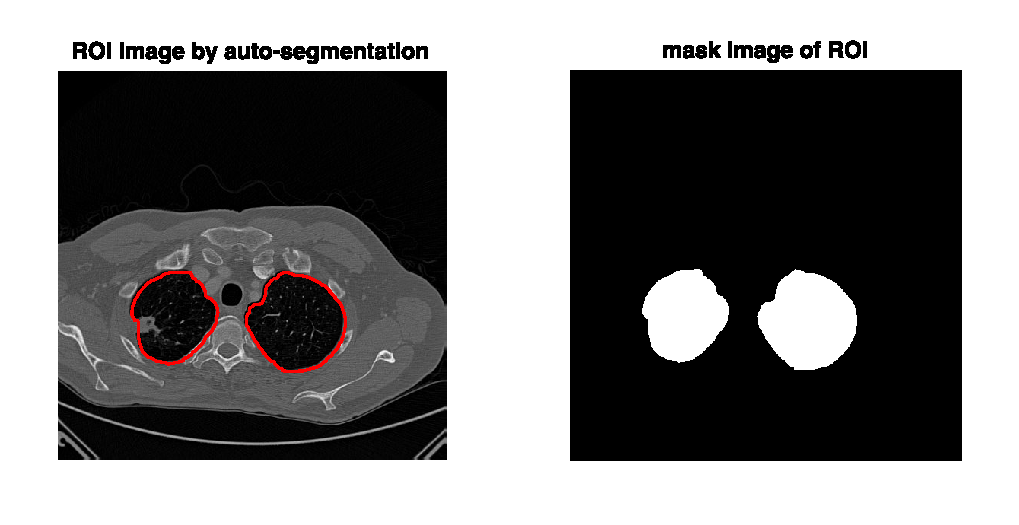
\includegraphics[width=1\linewidth]{ROI}
	\caption{Illustration of ROI in CT image. left: boundary of ROI. right: mask of lung region}
	\label{ROI}
\end{figure}
\\

\section{PERFORMANCE MEASURES}
We used four quality measures to evaluate our algorithm: signal-to-noise ratio, mean square error, peak signal-to-noise ratio and tamper assessment factor. Six common kinds of attacks in medical images were applied to test the watermarking performance.\\

\subsection{Signal-to-noise ratio (SNR)}
The SNR is used to estimate the noise of a signal in decibels. We take the original CT image as the signal and the deference between the processed image and the original one as the noise. SNR calculates the ratio of summed squared magnitude of the signal to that of the noise.
\[\ SNR(dB) = 10 log_{10} \frac{P_{Im}}{P_n}\]
Where $P_Im$ means the signal power and $P_n$ means the noise power.\\

\subsection{Mean squared error (MSE)}
The MSE is a measure of the quality of an estimator, which is defined as the average of the squares of the errors.
\[\ MSE = \frac{1}{M * N} \sum_{x=1}^{N}\sum_{y=0}^{M}(f(x,y)-Im(x,y))^2\]
Where $f(x,y)$ means the processed image, $Im(x,y)$ means the original image, $M$ and $N$ mean the width and the height of the image.\\

\subsection{Peak signal-to-noise ratio (PSNR)}
The PSNR is a ratio between the maximum possible power of a signal and the power of corrupting noise that affects the fidelity of its representation. PSNR is most commonly used in image reconstruction quality measurements, which is an approximation to human perception of image quality. PSNR is most easily defined via the MSE.
\[\ PSNR(dB) = 10 log_{10} \frac{MaxBits}{MSE}\]
Where $MaxBits$ stands for the maximum possible pixel value of the image.\\

\subsection{Tamper Assessment Factor (TAF)}
The TAF is an estimator of the error between the actual embedded watermark and the retrieved water mark. We embedded the known logo image into the diagonal detail of the first wavelet decomposition level and retrieved it. By calculating the deference between the actual watermark and the retrieved one.
\[\ TAF(w,w') = \frac{1}{M * N} \sum_{x=1}^{N}\sum_{y=0}^{M}(w(x,y)\oplus w'(x,y))\]
Where $w(x,y)$ means the original watermark, $w'(x,y)$ means the retrieved watermark, $M$ and $N$ mean the width and the height of the watermark image.\\

\section{RESULTS}

\section{FUTURE STEPS}


\addtolength{\textheight}{-12cm}   % This command serves to balance the column lengths
                                  % on the last page of the document manually. It shortens
                                  % the textheight of the last page by a suitable amount.
                                  % This command does not take effect until the next page
                                  % so it should come on the page before the last. Make
                                  % sure that you do not shorten the textheight too much.

%%%%%%%%%%%%%%%%%%%%%%%%%%%%%%%%%%%%%%%%%%%%%%%%%%%%%%%%%%%%%%%%%%%%%%%%%%%%%%%%



%%%%%%%%%%%%%%%%%%%%%%%%%%%%%%%%%%%%%%%%%%%%%%%%%%%%%%%%%%%%%%%%%%%%%%%%%%%%%%%%



%%%%%%%%%%%%%%%%%%%%%%%%%%%%%%%%%%%%%%%%%%%%%%%%%%%%%%%%%%%%%%%%%%%%%%%%%%%%%%%%
\section*{ACKNOWLEDGMENT}

SPIE-AAPM Lung CT Challenge

\begin{thebibliography}{99}
 \bibitem{c1} 
%\bibitem{c1} G. O. Young, ?Synthetic structure of industrial plastics (Book style with paper title and editor),? 	in Plastics, 2nd ed. vol. 3, J. Peters, Ed.  New York: McGraw-Hill, 1964, pp. 15?64.
%\bibitem{c2} W.-K. Chen, Linear Networks and Systems (Book style).	Belmont, CA: Wadsworth, 1993, pp. 123?135.
%\bibitem{c3} H. Poor, An Introduction to Signal Detection and Estimation.   New York: Springer-Verlag, 1985, ch. 4.
%\bibitem{c4} B. Smith, ?An approach to graphs of linear forms (Unpublished work style),? unpublished.
%\bibitem{c5} E. H. Miller, ?A note on reflector arrays (Periodical style?Accepted for publication),? IEEE Trans. Antennas Propagat., to be publised.
%\bibitem{c6} J. Wang, ?Fundamentals of erbium-doped fiber amplifiers arrays (Periodical style?Submitted for publication),? IEEE J. Quantum Electron., submitted for publication.
%\bibitem{c7} C. J. Kaufman, Rocky Mountain Research Lab., Boulder, CO, private communication, May 1995.

\end{thebibliography}


\end{document}
